\chapter{計時器與記分板}
\renewcommand{\baselinestretch}{10.0} %設定行距
\pagenumbering{arabic} %設定頁號阿拉伯數字
\setcounter{page}{8}  %設定頁數
\fontsize{14pt}{2.5pt}\sectionef
\section{摘要}
  完成球員設定後,接著說明場景中計時器設定與 LED 記分板和機械式轉盤記分板製作過程。\\
\section{計時器}
\begin{figure}[hbt!]
\begin{center}
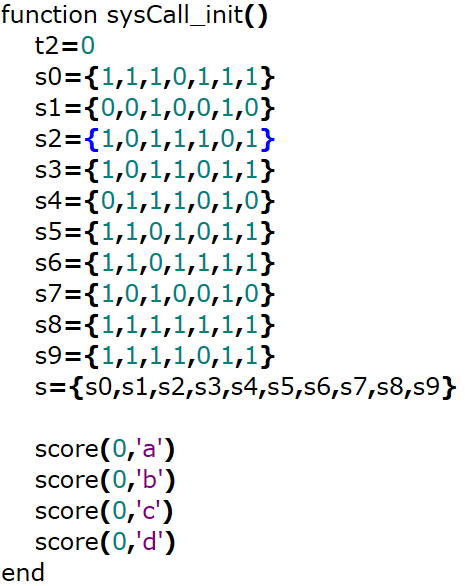
\includegraphics[height=8cm]{46}
\caption{\Large 定義變量}\label{fig.46}
\end{center}
\end{figure}
(圖.\ref{fig.46}) 以函數 sysCall init 定義一些變量,將 t2 初始化為 0,s0 到 s9 由 0 到 1 組成的列表,用於後續計算。通過調用 score(0, 'a')、score(0, 'b')、score(0, 'c')和 score(0, 'd') 來初始化名為 a、b、c、d 的得分。\\
  此程式碼做用是在模擬環境初始化階段定義一些變量、列表及得分的部分。\\
\newpage
\begin{figure}[hbt!]
\begin{center}
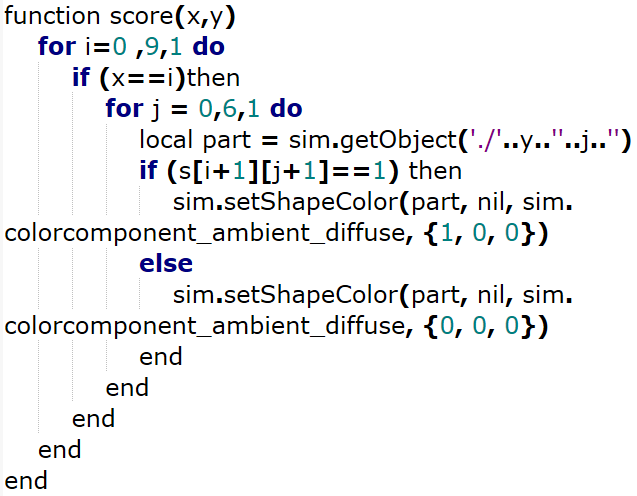
\includegraphics[height=8cm]{47}
\caption{\Large 數字顏色}\label{fig.47}
\end{center}
\end{figure}
(圖.\ref{fig.47}) score 函數接受參數 "x"、"y",使用一個循環重複數字 0 到 9,首先檢查"x"是否等於當前數字,如果相等則執行內部循環。以 sim.getObject() 根據給定的字符串構建對象名稱並儲存在 part 變量中。再檢查 s[i+1][j+1] ,數字 i 在位置 j 上如果為 1 就使用 sim.setShapeColor() 將 part 對象的顏色設置為紅色 ({1, 0, 0}),若非則將顏色設置為黑色 ({0, 0, 0})。\\
  根據輸入的數字"x"、"y"設置對應數字的顏色,以數字的模式在模擬環境中的相對應位置設置不同的顏色。\\
\newpage
\begin{figure}[hbt!]
\begin{center}
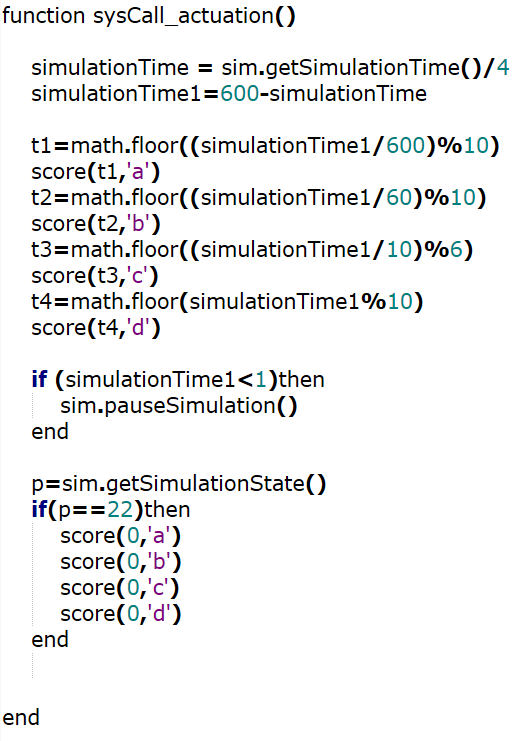
\includegraphics[height=9cm]{48}
\caption{\Large 更改數字形狀的顏色}\label{fig.48}
\end{center}
\end{figure}

(圖.\ref{fig.48}) sysCall actuation 在模擬時被調用,首先藉由 sim.getSimulationTime() 獲取當前時間並除以4,儲存在變量 simulationTime 中。以 simulationTime 計算"t1"、"t2"、"t3"及"t4",分別表示當前時間的不同部分,所得值通過 simulationTime1 除以相對應數字,並取整數部分。\\
再來以 score() 將計算得到的值分別與"a"、"b"、"c"、"d"一起傳遞,可以根據時間的變化來更新相應的數字形狀的顏色。\\
  根據模擬時間的變化更新數字形狀的顏色,在特定條件下暫停模擬或重置顯示的顏色。\\
\begin{figure}[hbt!]
\begin{center}
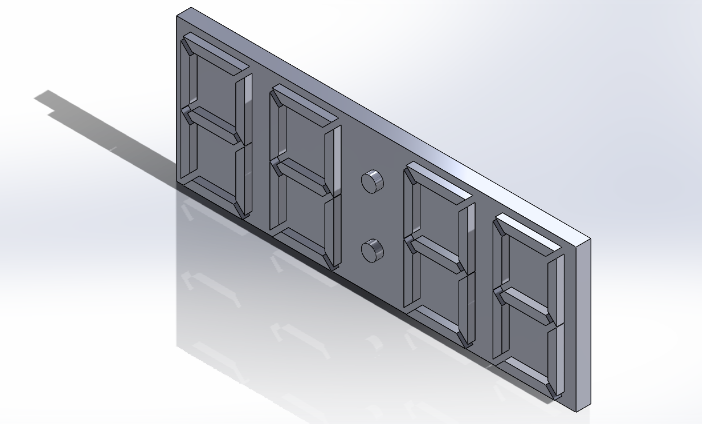
\includegraphics[width=6cm]{49}
\caption{\Large 計時器}\label{fig.49}
\end{center}
\end{figure}
\newpage
\section{LED記分板}
\begin{figure}[hbt!]
\begin{center}
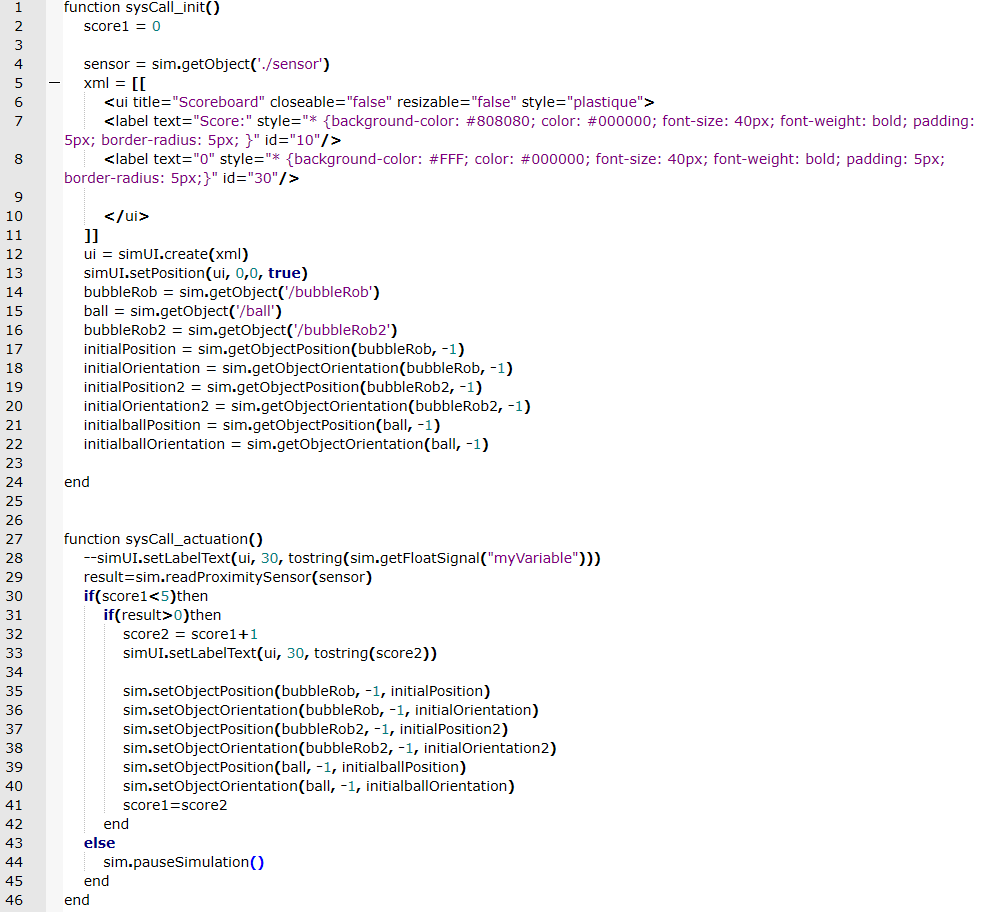
\includegraphics[width=16cm]{50}
\caption{\Large 記分板}\label{50}
\end{center}
\end{figure}
透過 Lua 程式建立記分板,設計樣式,給予偵測定義。\\
\newpage
\begin{figure}[hbt!]
\begin{center}

\includegraphics[width=16cm]{51}
\caption{\Large sensor}\label{fig.51}
\end{center}
\end{figure}

(圖.\ref{fig.51})sysCall init 的函式建立了一個名為 score1 的變數,並將它的值設定為 0使用 sim.getObject 方法來獲取一個名為 sensor 的物件,並將它儲存在 sensor 變數中。\\
\begin{figure}[hbt!]
\begin{center}
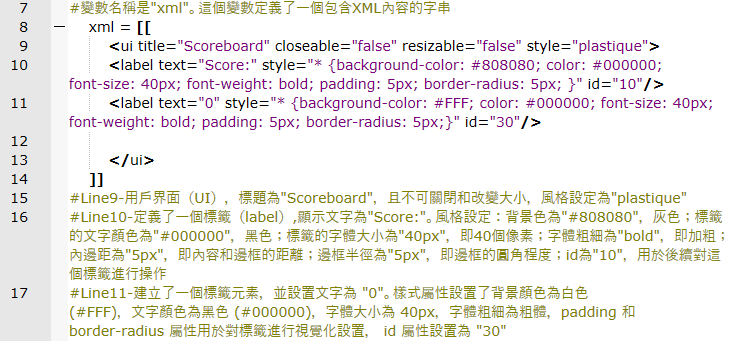
\includegraphics[width=16cm]{52}
\caption{\Large xml}\label{fig.52}
\end{center}
\end{figure}

(圖.\ref{fig.52}存儲在名為 xml 的變數中的 XML 代碼,它描述了一個顯示得分的視窗界面。ui 標籤中,有兩個 label 標籤,分別用來顯示 "Score:" 和得分。\\
\begin{figure}[hbt!]
\begin{center}
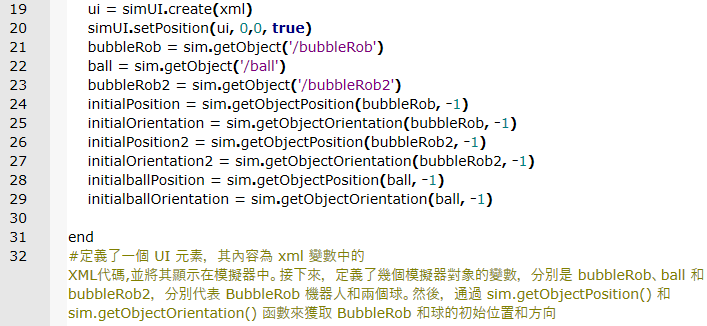
\includegraphics[width=16cm]{53}
\caption{\Large ui}\label{fig.53}
\end{center}
\end{figure}

\newpage
(圖.\ref{fig.53}建立使用者介面 (ui),然後設定該介面的位置為 (0, 0)。sim.getObject 函式從仿真場景中取得了三個物體,sim.getObjectPosition 和 sim.getObjectOrientation 函式取得了這些物體的初始位置和初始方向,這段程式碼是用來建立仿真場景中物體的初始位置和初始方向。\\
\begin{figure}[hbt!]
\begin{center}
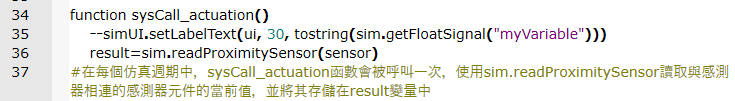
\includegraphics[width=16cm]{54}
\caption{\Large syscall}\label{fig.54}
\end{center}
\end{figure}

(圖.\ref{fig.54}sysCall-actuation的函式使用 sim.readProximitySensor 函式讀取一個接近傳感器的數據,並將結果儲存在 result 變數中。\\
\newpage
\begin{figure}[hbt!]
\begin{center}
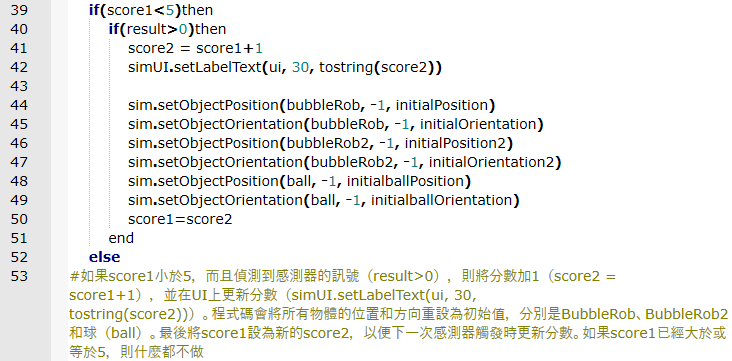
\includegraphics[width=16cm]{55}
\caption{\Large if-else}\label{fig.55}
\end{center}
\end{figure}

(圖.\ref{fig.55}這段程式碼的主要作用是檢查分數是否小於5分,如果 score1 的值小於5,且 result 大於0,則將分數加1並在ui上更新分數。如果 score1 的值已經達到或超過了5分,則會跳過。\\
\begin{figure}[hbt!]
\begin{center}
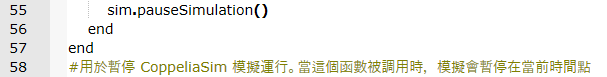
\includegraphics[width=16cm]{56}
\caption{\Large pause}\label{fig.56}
\end{center}
\end{figure}

(圖.\ref{fig.56}檢查分數是否小於5分。如果分數達到5分或更高,它會暫停仿真並結束程式執行。\\
\newpage
\section{機械式轉盤記分板}
  除了採用 LED 顯示計分外,另外建立以機械轉盤傳動計分系統,納入每按一下"i"轉盤及順時鐘旋轉36度。\\
\begin{figure}[hbt!]
\begin{center}
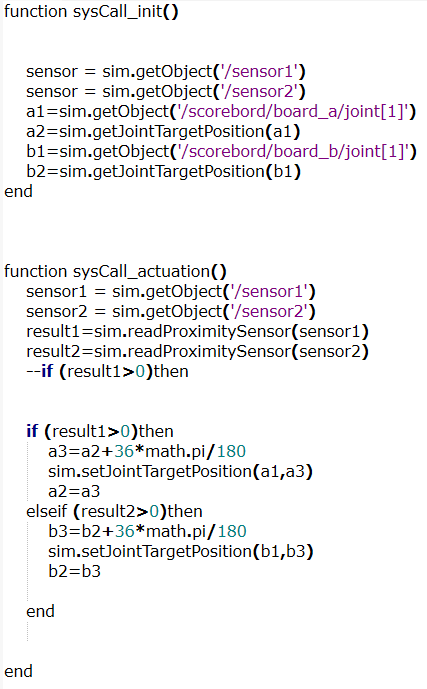
\includegraphics[width=9cm]{57}
\caption{\Large 機械記分板}\label{fig.57}
\end{center}
\end{figure}
\newpage
\begin{figure}[hbt!]
\begin{center}
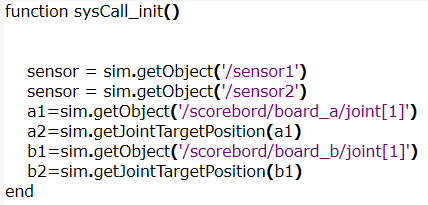
\includegraphics[width=8cm]{58}
\caption{\Large 獲取變量}\label{fig.58}
\end{center}
\end{figure}
(圖.\ref{fig.58} 使用 sim.getObject() 獲取 /sensor1 存入變量"sensor"、獲取 /scorebord/board a/joint[1] 的關節存入變量"a1",以 sim.getJointTargetPosition() 獲取"a1"目標位置存入變量"a2",獲取變量"b1"目標位置存入變量"b2"。\\
\begin{figure}[hbt!]
\begin{center}
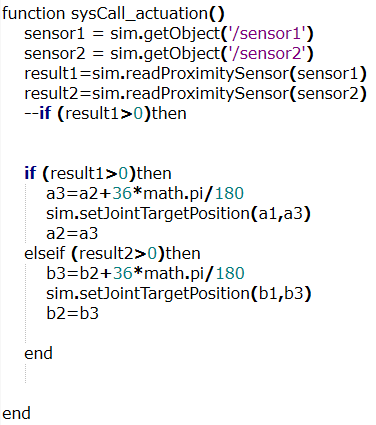
\includegraphics[width=6cm]{59}
\caption{\Large 角度偏移}\label{fig.59}
\end{center}
\end{figure}

(圖.\ref{fig.59} sim.readProximitySensor() 函數獲取近接傳感器 "sensor1"、"sensor2"的結果,存入變量"result1"、"result2",如果大於0則執行:關節"a1"的目標位置為當前位置"a2"加上36度的角度偏移,並將"a2"更新為"a3"以便下次執行使用。\\
  此程式碼根據接近傳感器的檢測結果來控制關節運動,使機械式轉盤隨比分計分。\\
\renewcommand{\baselinestretch}{0} %設定行距